% 1977 年四川卷第三题：△ABC 的外接园，AD、BD 为角平分线，
% AD 延长交园于 E，BD 延长交园于 F，求证 BE=DE；
% 弧上记号：1（弧BE）、2（弧EC）、3（弧CF）、4（弧AF）（按源卷第 3 页布局）
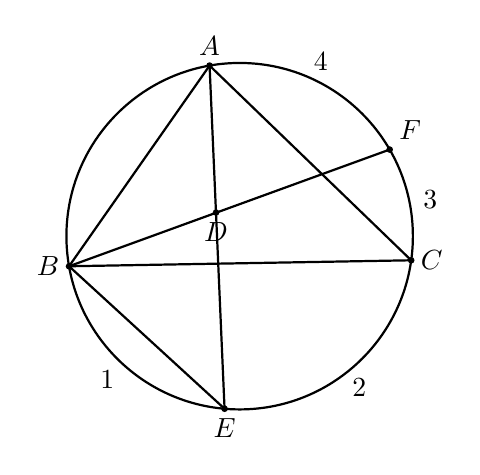
\begin{tikzpicture}[scale=1.0]
  \coordinate (A) at (100:2.2);
  \coordinate (F) at (30:2.2);
  \coordinate (C) at (-8:2.2);
  \coordinate (E) at (265:2.2);
  \coordinate (B) at (190:2.2);
  \coordinate (D) at (-0.30,0.30); % AE 与 BF 的交点
  \draw[thick] (0,0) circle (2.2);
  \draw[thick] (A)--(B)--(C)--cycle;
  \draw[thick] (A)--(E);
  \draw[thick] (B)--(F);
  \draw[thick] (B)--(E);
  \fill (A) circle (1.2pt) node[above] {$A$};
  \fill (B) circle (1.2pt) node[left] {$B$};
  \fill (C) circle (1.2pt) node[right] {$C$};
  \fill (D) circle (1.2pt) node[below] {$D$};
  \fill (E) circle (1.2pt) node[below] {$E$};
  \fill (F) circle (1.2pt) node[above right] {$F$};
  \node at (-1.68,-1.82) {$1$};
  \node at (1.52,-1.92) {$2$};
  \node at (2.42,0.46) {$3$};
  \node at (1.03,2.22) {$4$};
\end{tikzpicture}
